\subsection{Ram uitwerken en ontwerpen}
Om ons doel te bereiken om ballen te verzamelen en naar een zelf geselecteerde hoek te brengen hebben wij een enkel paar aanpassingen toepassen aan de buitenkant van de Zumo \cite{Zumo-bot}.\\

\begin{figure}[H]
    \centering
    \includegraphics[width=250pt]{img/zumo-mount.png}
    \caption{Zumo mount}
    \label{fig:zumo-mount}
\end{figure}

Een van deze aanpassingen was een grote vork aan de voorkant plaatsen, de binnenkant van deze vork spant 7.5cm wijdt, dit is ongeveer 1 cm groter dan de officiële diameter van een tennisbal (6,54cm - 68,6cm). Door deze marge toe te passen was het iets gemakkelijker om de tennisballen op te rapen. Tevens zit er een camera houder aan de voorkant van de vork gemonteerd. \\

Een andere aanpassing die we hebben toegevoegd is een shield voor de Arduino Uno \cite{Arduino-Uno}. In dit shield zijn 4 plusjes uitgesneden waarmee we de houder voor de Raspberry Pi \cite{Raspberry-Pi} in kunnen zetten. Dit kan gedaan worden zonder dat er schroefjes zijn die de onderkant van de Raspberry Pi raakt en mogelijk kortsluiting laat ontstaan. Verder hebben we aan de voorkant van het shield een extra montage mogelijkheid voor de vork geplaatst.\\

Als laatste aanpassing hebben we een Raspberry Pi houder toegevoegd, deze houder kan je monteren door middel van 4 plusjes die aan de de onderkant van de houder zitten het shield van de Arduino in te duwen. De Raspberry Pi zelf kan monteerd worden door schroefjes door het bord te doen en deze door de gleuven van de houder vast te monteren.

\subsection{Tennis ball model trainen}
Om te testen of we een eigen model beter zou zijn, hebben we eerst een eigen model getraind en deze getest tegen de COCO-dataset \cite{COCO-dataset} model.\\

Voor het trainen van het model had Sergi grofweg 500 afbeeldingen van tennisballen gedownload en gelabeld. Zoals te zien in figuur \ref{fig:model-verschil}, werkte de detectie net wat beter dan die van de COCO-dataset.\\

\begin{figure}[H]
    \begin{subfigure}{0.5\textwidth}
        \includegraphics[width=0.9\linewidth]{img/coco_model_test.png} 
        \caption{COCO-dataset model}
        \label{fig:coco-model}
    \end{subfigure}
    \begin{subfigure}{0.5\textwidth}
        \includegraphics[width=0.9\linewidth]{img/custom_model_test.png}
        \caption{Zelf getraind model}
        \label{fig:custom-model}
    \end{subfigure}
    \caption{Het verschil tussen het voorgetraind en het zelf getrainde model.}
    \label{fig:model-verschil}
\end{figure}

Er is er bij \ref{fig:custom-model} te zien dat niet alle ballen worden gedetecteerd, maar dat is in ieder geval beter dan het skateboard dat bij \ref{fig:coco-model} zou worden gedetecteerd. We zijn toen tot de conclusie gekomen dat een zelf getraind model beter was, aangezien er dan geen verwarring plaats kan vinden. Echter bleek wel dat het zelfgetrainde model meer moeite had met verschillende belichting. Er is toen voor gekozen om het dubbele aantal afbeeldingen te trainen. Dit zorgde er voor dat de detectie wat beter werkte en elke bal snel detecteerde. De focus lag dan ook vooral op ballen die ver weg -- en daardoor niet even scherp -- waren. In figuur \ref{fig:hall-way-ball} is een slecht belichte foto op 10 meter afstand genomen. De detectie is niet perfect, maar werkt nog redelijk goed. \\

\begin{figure}[H]
    \centering
    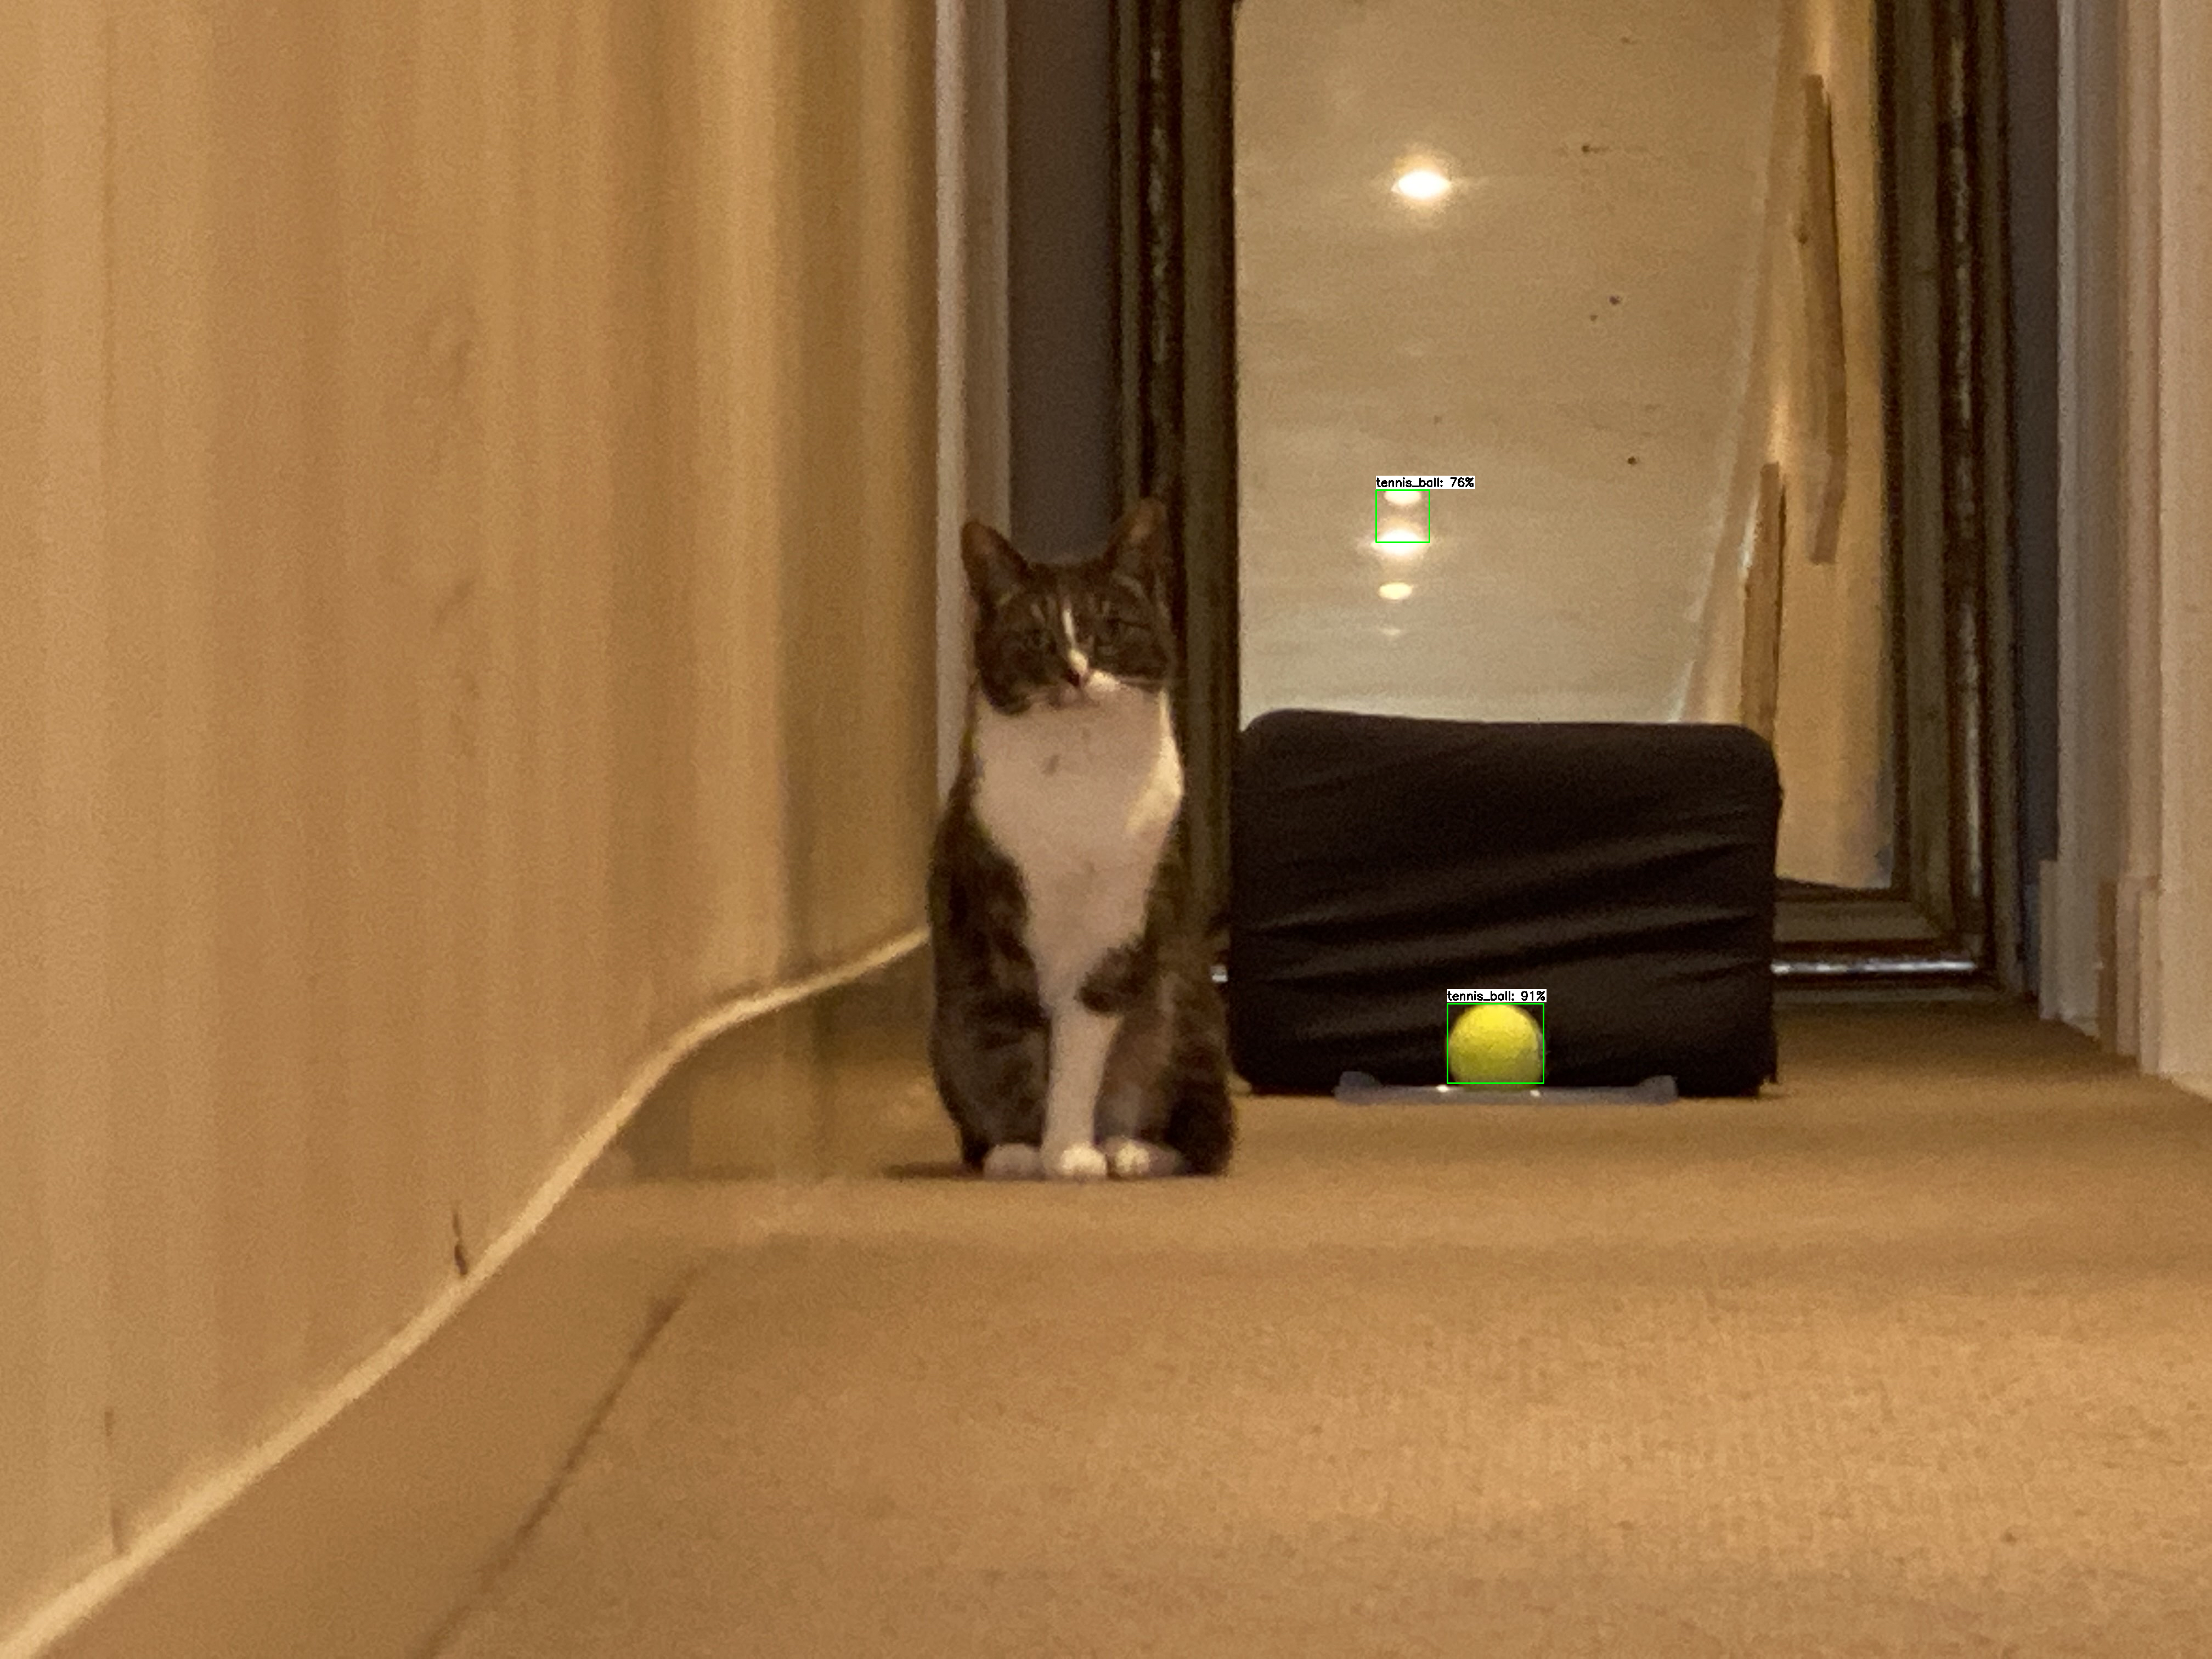
\includegraphics[width=250pt]{img/hall-way-ball.png}
    \caption{Een bal op 10 meter afstand, in een slecht belichte gang.}
    \label{fig:hall-way-ball}
\end{figure}

Er is veel getraind op afbeeldingen die \quotes{out of focus} waren. Echter hadden we niet door dat hierdoor het model vrijwel alles wat geel was zou detecteren als een tennisbal. Om dit tegen te gaan zijn we gebruik gaan maken van hard-negatives. Dit zijn objecten die je expliciet markeert als niet-juist. Dit zou er voor moeten zorgen dat er tijdens het trainen meer rekening wordt gehouden met de ronde vorm van een tennisbal. In figuur \ref{fig:model-hard-negative} is te zien dat de objecten niet als tennisballen worden gedetecteerd.

\begin{figure}[H]
    \begin{subfigure}{0.5\textwidth}
        \includegraphics[width=0.9\linewidth]{img/hard_negative_white.png} 
        \caption{COCO-dataset model}
        \label{fig:hard-negative-white}
    \end{subfigure}
    \begin{subfigure}{0.5\textwidth}
        \includegraphics[width=0.9\linewidth]{img/hard_negative_shoes.png}
        \caption{Zelf getraind model}
        \label{fig:hard-negative-shoes}
    \end{subfigure}
    \caption{Objecten die door de hard-negative training niet als tennisballen worden gezien.}
    \label{fig:model-hard-negative}
\end{figure}

Waar ik achteraf achter kwam  was dat de hard-negatives weer iets te veel op de witte achtergrond hadden getraind. Dit resulteerde er in dat objecten die op tennisballen leken met een groene achtergrond, alsnog als tennisballen werden gedetecteerd. In Figuur \ref{fig:false-positive} is hier een voorbeeld van te zien.

\begin{figure}[H]
    \centering
    \includegraphics[width=250pt]{img/hard_negative_background.png}
    \caption{False positive}
    \label{fig:false-positive}
\end{figure}

\subsection{Web-applicatie bouwen voor het instellen en lezen van de positie van de robot}
Voor de web-applicatie was eerst een design gemaakt in Figma. Dit is gedaan omdat we vooraf niet wisten wat de beste manier zou zijn geweest om de robot te bedienen. Uiteindelijke zijn we op een ontwerp gekomen waarin de gebruiker kan kiezen tussen drie verschillende modus:\\
\begin{enumerate}
    \item Terug naar het verzamel punt: Dit kan worden gebruikt als de tennisser wil spelen en de robot niet in de weg wil hebben. De robot zal niet verzamelen.
    \item Verzamel geselecteerde zone: De robot zal de ballen verzamelen in de geselecteerde zone. Dit is handig als er veel ballen achter de achterlijn liggen na een training.
    \item Verzamel overal: Deze modus kan worden gebruikt na afloop van het trainen. De robot zal dan rustig over heel het velt gaan om de ballen te verzamelen.
\end{enumerate}

Onder de drie knoppen voor de modus is een raster afgebeeld die grofweg een tennisveld representeert (er wordt geen rekening gehouden met dubbele lijnen). Het idee hiervan is dat de zones en het verzamelpunt kunnen worden aangegeven.\\

De uiteindelijke implementatie is geschreven in React \cite{React}, hier is voor gekozen, omdat we een goed werkende web-applicatie wilde, die niet al te veel boilerplate code had, zodat ontwikkelen sneller ging.\\

React heeft er uiteindelijk voor gezorgd dat het gebruik van de applicatie heel soepel verloopt. Zo kan er alleen een zone worden geselecteerd als de verzamelmodus aanstaat. Wel kan er altijd een verzamelpunt worden ingesteld. Op deze manier kan de robot in mode 1 alsnog van hoek naar hoek reizen. De manier waarop de huidige modus wordt aangegeven is door de velden op het raster aan te passen in hoe ze er uit zien en werken. Als de robot terug naar het verzamelpunt moet, worden alle zones een doffe kleur en zijn de knoppen disabled. In de verzamelmodus zal met een rand worden aangegeven welke zone wordt verzameld. In Figuur \ref{fig:web-app-modues} zijn de drie verschillende modus te zien.

\begin{figure}[H]
    \begin{subfigure}{0.3\textwidth}
        \includegraphics[width=0.9\linewidth]{img/mode-1.png} 
        \caption{Terug naar het verzamel punt}
        \label{fig:mode1}
    \end{subfigure}
    \begin{subfigure}{0.3\textwidth}
        \includegraphics[width=0.9\linewidth]{img/mode-2.png}
        \caption{Verzamel geselecteerde zone}
        \label{fig:mode2}
    \end{subfigure}
        \begin{subfigure}{0.3\textwidth}
        \includegraphics[width=0.9\linewidth]{img/mode-3.png}
        \caption{Verzamel overal
        \newline}
        \label{fig:mode3}
    \end{subfigure}
    \caption{De drie verschillende modus van de web-app.}
    \label{fig:web-app-modues}
\end{figure}

\subsection{Ballen detecteren en positie verkrijgen}
Voor het detecteren van de ballen wordt gebruik gemaakt van OpenCV \cite{OpenCV} en Tensorflow Lite \cite{Tensorflow-Lite} in combinatie met de Google Coral \cite{Google-Coral}. Het script dat we hebben gemaakt is voor een groot gedeelte gebaseerd op het script van EdjeElectronics \cite{EdjeElectronics}. Hij heeft een tutorial gemaakt voor het maken van Tensorflow Lite modellen. Het script is aangepast om geen visuele output te geven. Dit maakt de detectie al wat sneller. Daarnaast zijn er wat instellingen voor de video opname aangepast, zodat dit voor meer frames kan zorgen. Hiernaast hebben we alles omgezet in OOP. Dit maakte het vervolgens wat makkelijker om het script in de rest van de applicatie te integreren. Ook hebben we een pauzeer functie toegevoegd die de detectie kan pauzeren. De resultaten van de object detectie worden in een detectie object gezet. Dit object rekent de positie en afstand uit en zet deze in variabelen. De manier waarop dat gedaan wordt, is door de twee hoeken van het vierkant te pakken en van elkaar af te trekken, waardoor de breedte over blijft. Als deze breedte dan voor de helft van het meest rechtse punt wordt afgetrokken, blijft de positie van het midden van de detectie over. De functie die dit doet is te zien in figuur \ref{fig:get_width_and_position}.\\ 

\begin{figure}[H]
    \centering
    \begin{minted}{python}
    def get_width_and_position(boxes):
        xmin = boxes[1]
        xmax = boxes[3]
    
        width = (xmax - xmin)
        position = xmin + (width / 2)
    
        return width, position
    \end{minted}
    \caption{Functie om de breedte en positie van een detectie te bepalen.}
    \label{fig:get_width_and_position}
\end{figure}

\subsection{Bepaal welke bal het dichtstbij is door de breedte uit te rekenen}
Om uit de detectie de bal terug te krijgen die het meest dichtbij is wordt gebruik gemaakt van de breedte die voorheen is berekent. Je zou namelijk kunnen zeggen dat een bal die dichterbij ligt, er breeder uit ziet op het beeld. In python zit een functie die het erg makkelijk maakt om de grootste waarde terug te krijgen. De functie die de juiste detectie terug geeft is erg Pythonic geschreven en is te zien in figuur \ref{fig:get_nearest_detection}.\\

\begin{figure}[H]
    \centering
    \begin{minted}{python}
    def get_nearest_detection(detections):
        detection = max(detections, key=lambda d: d.width)
        return detection
    \end{minted}
    \caption{Functie om de dichtbije detectie te krijgen.}
    \label{fig:get_nearest_detection}
\end{figure}

\subsection{Backend voor de web-appplicatie maken}
De backend van de web-applicatie wilde we zo simpel en snel mogelijk maken. Om voor makkelijke integratie te zorgen hebben we er voor gekozen mo de webserver met Flask \cite{Flask} te maken. Op deze manier hoeft er maar een programma gedraaid te worden op de Raspberry Pi. De Flask webserver beschikt over drie variabelen:\\

\begin{enumerate}
    \item zone: De zone waarin verzameld wordt.
    \item collection: Het verzamelpunt.
    \item collection\_mode: De verzamelmodus van de robot.
\end{enumerate}

Voor elk van deze variabelen is een endpoint die een GET of POST request verwacht. Aan de hand van de soort request zal de webserver de variabele terug geven of opslaan. In figuur \ref{fig:handle_zone} is te zien hoe zo'n endpoint er uit ziet.\\

\begin{figure}[H]
    \centering
    \begin{minted}{python}
    @app.route(ZONE_URI, methods=['GET', 'POST'])
    def handle_zone():
        global zone
        if is_post(request):
            zone = request.json['zone']
        return json.dumps(zone)
    \end{minted}
    \caption{Een Flask endpoint die variabelen kan zetten en teruggeven.}
    \label{fig:handle_zone}
\end{figure}

\subsection{Verbinding tussen Raspberry Pi en Arduino}
De verbinding tussen de Raspberry Pi en de Arduino wordt in stand gebracht door middel van een seriële (UART) verbinding op de baudrate 115200. In het onderzoek hadden we beschreven dat we I2C zouden gebruiken. Alleen daar zijn we op het laatste moment van af geweken doordat het weinig extra functionaliteit meer bood in onze use-case en het complexer was om op te zetten op de Raspberry Pi. \\

Voor de seriële verbinding van de Pi wordt er gebruik gemaakt van de library \quotes{pyserial}. Deze library maakt het mogelijk om gemakkelijk naar de seriële buffer van de Arduino te schrijven. Voor de rest hadden we een kleine \quotes{service} gemaakt in het Python script die gebruik maakte van een lock. Door het gebruik van een lock was het niet meer mogelijk om met meerdere threads naar dezelfde buffer te schrijven, hierdoor was het niet meer mogelijk dat er een race-condition ontstond aan de Python kant.\\

Voor de seriele verbinding van de Arduino wordt de standaard libary gebruikt die Arduino automatisch meelevert in Arduino projecten. Iedere \quotes{tick} van de Zumo wordt er gekeken of er iets in geschreven is. Zo ja, kijk of het een commando is en voer deze uit.\\

Iedere opdracht die opgestuurd wordt naar de Zumo moet zich houden aan de voor gespecificeerde notatie. De notatie ziet er zo uit: \quotes{commando=argument;}. Waarbij het commando de naam moet zijn van de opdracht die je wilt doen het argument een waarde moet zijn die de werking van de opdracht beïnvloed. Alle mogelijke commando's staan in de tabel hieronder beschreven. 

\begin{figure}[H]
    \begin{tabularx}{\textwidth}{|l|l|X|}
        \hline
        \rowcolor[HTML]{C0C0C0} Commando & Argument & Beschrijving \\\hline
        move & [-400, 400] & Beweegt beide tracks dezelfde richting in. \\\hline
        left & [-400, 400] & Beweegt 1 track de gewenste richting in. \\\hline
        right & [-400, 400] & Beweegt 1 track de gewenste richting in. \\\hline
        center-left & [-400, 400] & Beweegt linksom rond z'n eigen as. \\\hline
        center-right & [-400, 400] & Beweegt rechtsom rond z'n eigen as. \\\hline
        honk & - & Maakt een \quotes{honk} geluid. \\\hline
        stop & - & Stopt beide tracks. \\\hline
    \end{tabularx}
    \caption{Commandos van de Zumo}
    \label{fig:commands}
\end{figure}

\subsection{Lokale positie berekenen door middel van BLE}
Om de lokale positie te berekenen van de TennisBallBot wordt er gebruik gemaakt van beacons. Deze beacons ondersteunen het iBeacon protocol \cite{ibeacon} waarmee het mogelijk is de afstand te meten tussen de bot en de beacons. \\
\begin{figure}[H]
    \centering
    \includegraphics[width=200pt]{img/beacon.png}
    \caption{Beacon die aan staat}
    \label{fig:beacon}3
\end{figure}

De afstand tussen de robot en de beacons wordt berekent door middel van RSSI (Recieved Signal Strength Indicator). Dit is een geschatte meting van hoe goed een apparaat een signaal ontvangt. De signaalwaarde wordt bij RSSI gemeten in decibel van 0 tot -120. Hoe dichter bij de 0 hoe sterker het signaal zou zijn. \\

\begin{figure}[H]
    \begin{subfigure}{0.5\textwidth}
        \centering
    
        \includegraphics[width=0.8\textwidth]{img/rssi_10cm_small.png} 
        \caption{RSSI op 10cm afstand}
        \label{fig:rssi_meting_10cm}
    \end{subfigure}
    \begin{subfigure}{0.5\textwidth}
        \centering
    
        \includegraphics[width=0.8\linewidth]{img/rssi_100cm_small.png} 
        \caption{RSSI op 100cm afstand}
        \label{fig:rssi_meting_100cm}
    \end{subfigure}
    \caption{RSSI metingen op verschillende afstanden.}
    \label{fig:RSSI_meting}
\end{figure}

Na wat testen kwamen wij er achter dat de RSSI van ons BLE signaal ongeveer in de buurt kwam van andere apparaten die een passief Bluetooth signaal uitzenden. Onze test resultaten waren in de buurt van -70db op ongeveer 5cm afstand tot ~-80db bij 1 meter, na ongeveer 3 meter was het signaal niet meer bruikbaar door te veel ruis. \\

Het zou eventueel mogelijk zijn om de signaalsterkte van de beacons te versterken door onder andere een betere antenne op de robot en/of beacons te zetten, of een sterker transmitter/ontvanger op de apparaten te plakken.\\

Als protocol voor de beacons hadden wij het iBeacon protocol geïmplementeerd, de hoofdredenen hiervoor is omdat het een gestandaardiseerd protocol is met de al ingebouwde functionaliteit om afstand te berekenen op basis van RSSI. De code die hier voor nodig is hieronder te zien. \\

\begin{figure}[H]
    \centering
    \begin{minted}{cpp}
    void create_beacon() {
        BLEBeacon beacon = BLEBeacon();
        beacon.setManufacturerId(0x4C00); // Fake Apple manufacturer id
        beacon.setProximityUUID(BLEUUID(resource_uuid));
        beacon.setMajor(resource_major);
        beacon.setMinor(resource_minor);
        beacon.setSignalPower(0xC1);
        
        BLEAdvertisementData advertisement_data = BLEAdvertisementData();
        BLEAdvertisementData scan_response_data = BLEAdvertisementData();
        
        advertisement_data.setFlags(0x04);
        
        std::string service_data = "";
        
        service_data += (char) 0x1A; // Len
        service_data += (char) 0xFF; // Type
        service_data += beacon.getData();
        
        advertisement_data.addData(service_data);
        
        ble_advertising->setAdvertisementData(advertisement_data);
        ble_advertising->setScanResponseData(scan_response_data);
}
    \end{minted}
    \caption{iBeacon implementatie op de beacons}
    \label{fig:beacon_code}
\end{figure}

Doordat we een gestandaardiseerd protocol hadden gebruikt voor de beacons was het mogelijk om een library te gebruiken voor het uitlezen van de beacons. De naam van deze Python3 library is \quotes{beacontools} \cite{beacontools} en maakt het mogelijk om gemakkelijk de advertise signalen van de beacons op te vangen en te verwerken. Met de data die wij ontvingen van de beacons hadden wij een simpele virtualisatie gemaakt. Deze virtualisatie toonde aan waar de robot dacht waar die op dat moment zou zijn op het veld. \\
\begin{figure}[H]
    \centering
    \includegraphics[width=200pt]{img/plotter.png}
    \caption{Virtualisatie van de positie van de robot}
    \label{fig:plotter}
\end{figure}

Een nadeel waar we achter kwamen was dat de enkele waardes van de beacon niet super accuraat waren, om een accurate positie te krijgen moesten je meerdere metingen hebben van dezelfde locatie. Hierdoor moesten we af en toe ~20 seconden wachten om genoeg waardes te krijgen van huidige locatie. Verder was het lastig om de positie te updaten als de robot aan het rijden was. Dit kwam omdat het niet echt mogelijk was om van een bewegende positie genoeg data te krijgen.\\

De uiteindelijke nauwkeurigheid die wij konden uitlezen van de robot zat in de buurt van de 20cm tot 5cm. Met hoe dichter de robot in het midden was hoe beter de nauwkeurigheid werd van de positie.

